\documentclass{article}




\usepackage{fullpage}
\usepackage{nopageno}
\usepackage{amsmath}
\usepackage{amsfonts}
\usepackage{graphicx}
\usepackage{framed}
\usepackage{algorithmic}
\usepackage{xcolor}

\definecolor{dark_red}{rgb}{0.5,0.0,0.0}
\definecolor{dark_green}{rgb}{0.0,0.5,0.0}
\definecolor{dark_blue}{rgb}{0.0,0.0,0.5}
\definecolor{blue}{rgb}{0.0,0.0,1.0}

\newcommand{\dr}[1]{\textcolor{dark_red}{#1}}
\newcommand{\dg}[1]{\textcolor{dark_green}{#1}}
\newcommand{\db}[1]{\textcolor{dark_blue}{#1}}
\newcommand{\blue}[1]{\textcolor{blue}{#1}}


\usepackage{fancyhdr}
%\setlength{\footheight}{15.2pt}
\pagestyle{fancy}
\fancyhead[C]{Wentworth Institute of Technology, MATH2025}
\fancyfoot[C]{Author: Shawn Eastwood}
\renewcommand{\headsep}{25pt}
\renewcommand{\headrulewidth}{1pt}
\renewcommand{\footrulewidth}{1pt}


\title{Mathematical notation review}
\date{}

\begin{document}

\maketitle

\section*{Sets}

Mathematics involves more than just numbers. In the topics that are covered in this class, a basic understanding of the notation related to ``sets" of entities is incredibly useful.  

\begin{itemize}
\item A ``set" is a collection of objects referred to as ``elements". Elements can be, but are not limited to, numbers.
\item Sets {\bf do not} contain duplicate elements (duplicate elements are ignored).
\item A set will be denoted by listing the elements enclosed by \(\{...\}\). The ordering of the elements does not matter. Duplicate elements are ignored.
\item The empty set is denoted by \(\emptyset\) or \(\{\}\).
\item Sets \(A\) and \(B\) are equal \(A = B\) if and only if \(A\) and \(B\) have the same elements. Every element of set \(A\) can be found in set \(B\) and vice versa.
\item \(x \in A\) if and only if \(x\) belongs to set \(A\). \(x \notin A\) if and only if \(x\) does not belong to set \(A\).
\end{itemize}

\textbf{Examples:}
\begin{itemize}
\item \(\{1, 6, 5\} = \{5, 1, 6\} = \{5, 1, 1, 6\}\)
\item \(2 \in \{4, 2, 3\}\)
\item \(5 \notin \{4, 2, 3\}\)
\end{itemize}

\textbf{Important sets of numbers:}
\begin{itemize}
\item ``natural numbers": \(\mathbb{N} = \{1, 2, 3, 4, ...\}\)
\item ``whole numbers": \(\mathbb{W} = \{0, 1, 2, 3, 4, ...\}\)
\item ``integers": \(\mathbb{Z} = \{..., -4, -3, -2, -1, 0, 1, 2, 3, 4, ...\}\)
\item ``rational numbers": \(\mathbb{Q}\) is the set of all numbers that are the division of two integers. 
\item ``real numbers": \(\mathbb{R}\) is the set of all numbers that are distances and their negatives. The set of real numbers contains the set of rational numbers.
\item ``irrational numbers": \(\mathbb{I}\) is the set of all real numbers that are not also rational. % = \mathbb{R} \setminus \mathbb{Q}\)
\end{itemize}

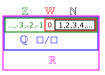
\includegraphics[width = 0.5\textwidth]{set_of_real_numbers}

\textbf{Examples:}

\begin{itemize}
\item Classify \(\sqrt{2}\): Irrational
\item Classify \(-4\): Integer, but not a whole number
\item Classify \(6/3\): Natural number
\item Classify \(0\): Whole number, but not a natural number
\item Classify \(-4/5\): Rational number, but not an integer
\item Classify \(100\): Natural number
\end{itemize}

How can large sets, or sets with an infinite number of elements be denoted? Here will be introduced {\bf set builder notation}. A set can be denoted by the syntax:
\[\{\dr{\text{expression}}|\dr{\text{condition}}\}\]
The ``\(\dr{\text{expression}}\)" is an algebraic expression, most often a single variable, whose attainable values form the elements of the set. The ``\(\dr{\text{condition}}\)" is a condition that must be satisfied for the value of the expression to count towards the set. The symbol ``\(|\)" reads as ``where".
%``Set builder" notation: \(\{x | \text{condition}(x)\}\) or \(\{x : \text{condition}(x)\}\) or \(\{x \in D | \text{condition}(x)\}\) or \(\{x \in D : \text{condition}(x)\}\)
To help denote conditions, the following notations will be used to shorten the description of conditions:

\begin{itemize}
\item Given conditions \(A\) and \(B\), \(A \wedge B\) denotes \(A\) ``AND" \(B\)
\item Given conditions \(A\) and \(B\), \(A \vee B\) denotes \(A\) ``OR" \(B\)
\item Given condition \(A\), \(\neg A\) denotes ``NOT" \(A\)
\item Given conditions \(A\) and \(B\), \(A \implies B\) denotes that the truth of \(A\) ``implies" the truth of \(B\) (\(A\) is true only if \(B\) is also true). This notation is important when solving equations. For example, \(x = 2 \implies x^2 = 4\). Also, \(x \geq 3 \implies x \geq 2\).
\item Given conditions \(A\) and \(B\), \(A \iff B\) denotes that \(A\) is true ``if and only if" (abbreviated by ``iff") \(B\) is true. \(A\) and \(B\) are either both true, or both false. This notation is important when solving equations. For example, \(x + 1 = 3 \iff x = 2\). Also, \(x^2 = 4 \iff ((x = 2) \vee (x = -2))\).
\item Given set \(A\) and condition \(B(x)\) (\(B(x)\) depends on \(x\)), the notation \(\forall x : B(x)\) denotes ``for all values of \(x\), \(B(x)\) is true". The notation \(\forall x \in A : B(x)\) denotes ``for all values of \(x\) from set \(A\), \(B(x)\) is true". For example, \(\forall x \in \mathbb{R} : (x + 1) - 1 = x\).
\item Given set \(A\) and condition \(B(x)\) (\(B(x)\) depends on \(x\)), the notation \(\exists x : B(x)\) denotes ``there exists a value of \(x\) such that \(B(x)\) is true". The notation \(\exists x \in A : B(x)\) denotes ``there exists a value of \(x\) from set \(A\) such that \(B(x)\) is true". For example, \(\exists x \in \mathbb{R} : x + 4 = 10\).
\end{itemize}

\textbf{Examples}
\begin{itemize}
\item The set of rational numbers \(\mathbb{Q}\) can be denoted by \(\mathbb{Q} = \{n/m | (n \in \mathbb{Z}) \wedge (m \in \mathbb{Z})\}\)
\item The set of even integers can be denoted by either \(\{2n | n \in \mathbb{Z}\}\) or by \(\{n | \exists m \in \mathbb{Z} : 2m = n\}\)
\item The set of odd integers can be denoted by either \(\{2n+1 | n \in \mathbb{Z}\}\) or by \(\{n | \neg\exists m \in \mathbb{Z} : 2m = n\}\)
\item The set of square integers can be denoted by either \(\{n^2 | n \in \mathbb{Z}\}\) or by \(\{n | \exists m \in \mathbb{Z} : m^2 = n\}\)
\end{itemize}

In many cases, when the values of the ``\dr{expression}" are to be limited to a set \(A\), the notation:
\[\{\dr{\text{expression}} \in A|\dr{\text{condition}}\}\]
replaces 
\[\{\dr{\text{expression}}| (\dr{\text{expression}} \in A) \wedge \dr{\text{condition}}\}\]




\subsection*{Set operators and relations}

\begin{itemize}
\item Sets \(A\) and \(B\) are equal if and only if \(A\) and \(B\) have the same elements: \(\forall x : (x \in A) \iff (x \in B)\)
\item Set \(B\) is a subset of set \(A\), denoted by \(B \subseteq A\), if and only if the elements of \(B\) can also be found in \(A\): \(\forall x : (x \in B) \implies (x \in A)\)
\item Set \(B\) is a proper subset of set \(A\), denoted by \(B \subset A\), if and only if \(B \subseteq A\) and \(B \neq A\)
\item The union of two sets \(A\) and \(B\) is a set that consists of the elements from both sets. Duplicate elements are not included. \(A \cup B = \{x | (x \in A) \vee (x \in B)\}\)
\item The intersection of two sets \(A\) and \(B\) is a set that consists of the elements that are common to both sets. \(A \cap B = \{x | (x \in A) \wedge (x \in B)\}\)
\item The ``set difference" between sets \(A\) and \(B\) consists of all elements of \(A\) that do not also appear in \(B\). \(A \setminus B = \{x | (x \in A) \wedge \neg(x \in B)\}\)
\item The number of unique elements in set \(A\) is denoted by \(|A|\).
\end{itemize}

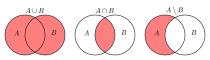
\includegraphics[width = \textwidth]{set_operations}

\textbf{Examples:}
\begin{itemize}
\item \(\{3, 4\} \subset \{4, 2, 3\}\)
\item \(\{3, 4\} \subseteq \{4, 2, 3\}\)
\item \(\{3, 4, 2\} \not\subset \{4, 2, 3\}\)
\item \(\{3, 4, 2\} \subseteq \{4, 2, 3\}\)
\item \(\{1, -1, 3\} \cup \{4, -2\} = \{1, -1, 3, 4, -2\}\)
\item \(\{1, -1, 4\} \cup \{4, -2\} = \{1, -1, 4, -2\}\)
\item \(\{1, -1, 4\} \cap \{4, -2\} = \{4\}\)
\item \(\{1, -1, 3\} \cup \emptyset = \{1, -1, 3\}\)
\item \(\{1, -1, 3\} \cap \emptyset = \emptyset\)
\item \(\{1, -1, 3\} \setminus \{4, -2\} = \{1, -1, 3\}\)
\item \(\{1, -1, 4\} \setminus \{4, -2\} = \{1, -1\}\)
\item \(|\{7, 2, 1\}| = 3\)
\item \(|\{1, 2, 1\}| = 2\)
\item \(|\emptyset| = 0\)
\end{itemize}

In many cases, the set of all real numbers between two bounds \(a\) and \(b\) needs to expressed in a compact manner. For this purpose interval notation is introduced. Given bounds \(a\) and \(b\) where \(a < b\),
\begin{itemize}
\item \((a, b) = \{x \in \mathbb{R} | a < x < b\}\)
\item \((a, b] = \{x \in \mathbb{R} | a < x \leq b\}\)
\item \([a, b) = \{x \in \mathbb{R} | a \leq x < b\}\)
\item \([a, b] = \{x \in \mathbb{R} | a \leq x \leq b\}\)
\end{itemize}



\subsection*{Tuples and vectors}

Given two values \(x\) and \(y\), an {\bf ordered pair} involving \(x\) and \(y\) is a 2 element list \(\langle x, y\rangle\) where \(x\) is the \(1^{\text{st}}\) or ``left" entry, and \(y\) is the \(2^{\text{nd}}\) or ``right" entry. As the name suggests, the order of the entries in an ordered pair is important. If \(x \neq y\), then \(\langle x, y \rangle \neq \langle y, x \rangle\).

Given sets \(A\) and \(B\), the ``set product" \(A \times B\) is the set of all possible ordered pairs that are formed by choosing the first entry from \(A\), and the second entry from \(B\): 

\[A \times B = \{\langle x, y \rangle | x \in A \wedge y \in B\}\]   

\textbf{Examples:}
\begin{itemize}
\item \(\{5, 6, 1\} \times \{0, 2\} = \{\langle 5, 0 \rangle, \langle 5, 2 \rangle, \langle 6, 0 \rangle, \langle 6, 2 \rangle, \langle 1, 0 \rangle, \langle 1, 2 \rangle\}\) 
\item \(\{1, 3\} \times \{0, 1, 3\} = \{\langle 1, 0 \rangle, \langle 1, 1 \rangle, \langle 1, 3 \rangle, \langle 3, 0 \rangle, \langle 3, 1 \rangle, \langle 3, 3 \rangle\}\) 
\item \(\{4, 2, -1\} \times \emptyset = \emptyset\)   
\item \(\{5, 0, 5\} \times \{0, 1, 1, 2\} = \{5, 0\} \times \{0, 1, 2\} = \{\langle 5, 0 \rangle, \langle 5, 1 \rangle, \langle 5, 2 \rangle, \langle 0, 0 \rangle, \langle 0, 1 \rangle, \langle 0, 2 \rangle\}\)
\end{itemize}

Given a list of \(n\) values \(x_1\), \(x_2\), ..., \(x_n\), the list \(\langle x_1, x_2, ..., x_n \rangle\) is often referred to as an ``\(n\)-tuple" (a generalization of the words double, triple, quadruple, etc.) or an \(n\) component vector. An ordered pair is simply a \(2\)-tuple. 

An \(n\)-tuple/vector can be denoted by either \(\langle x_1, x_2, ..., x_n \rangle\) or \(\begin{bmatrix} x_1 \\ x_2 \\ \vdots \\ x_n \end{bmatrix}\). Both representations are valid. The number of components \(n\) in a vector is referred to as the {\bf dimension} of said vector.

Given the \(n\) sets \(A_1, A_2, ..., A_n\), the set product \(A_1 \times A_2 \times ... \times A_n\) is the set of all \(n\) component vectors where the first entry is from \(A_1\), the second entry is from \(A_2\), the third entry is from \(A_3\) and so on:
\[A_1 \times A_2 \times ... \times A_n = \{\langle x_1, x_2, ..., x_n \rangle | x_1 \in A_1 \wedge x_2 \in A_2 \wedge ... \wedge x_n \in A_n\}\] 

The set \(A^n\) is the set of all \(n\) component vectors where the entries all come from \(A\):
\[A^n = \underbrace{A \times A \times ... \times A}_n = \{\langle x_1, x_2, ..., x_n \rangle | x_1 \in A \wedge x_2 \in A \wedge ... \wedge x_n \in A\}\]

The set of all \(n\) component vectors whose entries are real numbers is \(\mathbb{R}^n\). 

\textbf{Examples:}
\begin{itemize}
\item \(\mathbb{R}^2\) is the set of all 2D Cartesian coordinates.
\item \(\mathbb{R}^3\) is the set of all 3D Cartesian coordinates.
\end{itemize}



\section*{Functions}

Functions are mathematical objects that take values from a domain set \(X\) and with this value generate another value from a codomain set \(Y\). A function \(f\) with a domain of \(X\) and a codomain of \(Y\) is introduced by the notation:
\[f: X \rightarrow Y\]
The variable \(x\) that denotes the input value from \(X\) is often referred to as the ``input variable" or the ``parameter" of function \(f\). 
The value that is generated from the input value of \(x\), denoted by \(f(x)\), is often referred to as the ``output value" or the ``return value" from function \(f\).

The domain of a function \(f\) will be denoted by \(\textbf{domain}(f)\). The ``range" of function \(f\), denoted by \(\textbf{range}(f)\), is the set of all values from the codomain \(Y\) that are actually generated by some value from the domain \(\textbf{domain}(f)\):
\[\textbf{range}(f) = \{f(x) | x \in \textbf{domain}(f)\}\]    

If a function \(f\) is ``1 to 1", then no two different input values result in the same output value: 
\[\forall x_1, x_2 \in \textbf{domain}(f) : (x_1 \neq x_2 \implies f(x_1) \neq f(x_2))\]
Given a 1-to-1 function \(f\), then for each value \(y\) from the range of \(f\), there is exactly one input value \(x\) from the domain of \(f\) that returns \(y\). When a function \(f\) is ``1 to 1", the function \(f\) has an inverse. The inverse function of \(f\), denoted by \(f^{-1}\), ``reverses" function \(f\). The domain of \(f^{-1}\) is the range of \(f\), while the range of \(f^{-1}\) is the domain of \(f\). Given any value \(x\) from the range of \(f\), the value of \(f^{-1}(x)\) is the unique value from the domain of \(f\) such that \(f(f^{-1}(x)) = x\). For every value \(x\) from the domain of \(f\), applying \(f\) followed by \(f^{-1}\) brings \(x\) full circle: 
\[\forall x \in \textbf{domain}(f) : f^{-1}(f(x)) = x\]
For every value \(x\) from the range of \(f\), applying \(f^{-1}\) followed by \(f\) also brings \(x\) full circle:
\[\forall x \in \textbf{range}(f) : f(f^{-1}(x)) = x\] 

\textbf{Examples:}
\begin{itemize}
\item Let function \(f: [1, 2) \rightarrow \mathbb{R}\) be defined by \(f(x) = 2x + 3\). Note that even though the expression \(2x + 3\) is defined for all real values of \(x\), the domain of \(f\) has been artificially restricted to the interval \([1, 2)\). While the codomain of \(f\) is \(\mathbb{R}\), the range of \(f\) is \(\textbf{range}(f) = [5, 7)\). Function \(f\) is 1-to-1, and the inverse of \(f\) has a domain of \([5, 7)\) and a range of \([1, 2)\):
\[f^{-1} : [5, 7) \rightarrow [1, 2)\]  
moreover, \(f^{-1}(y) = \frac{y - 3}{2}\).
\item Let function \(g: \mathbb{R} \rightarrow \mathbb{R}\) be defined by \(g(x) = 5 - x^2\). The range of \(g\) is \(\textbf{range}(g) = (-\infty, 5]\). Function \(g\) is not 1-to-1, and so \(g\) does not have an inverse. If the domain of \(g\) were then artificially restricted to \((-\infty, -1)\), then the range is now \((-\infty, 4)\), and \(g\) becomes 1-to-1. The inverse function \(g^{-1} : (-\infty, 4) \rightarrow (-\infty, -1)\) is \(g^{-1}(y) = -\sqrt{5 - y}\).  
\end{itemize}

Multivariable calculus studies functions \(f\) whose domains are sets of vectors, and whose codomains are also sets of vectors:
\[f: \mathbb{R}^m \rightarrow \mathbb{R}^n\]   

When the domain of a function is a set of vectors with 2 or more components/dimensions, the function is referred to as being {\bf multivariable}. For a multivariable function, components of the input vector can be treated as separate parameters. Consider for example a function \(f: \mathbb{R}^2 \rightarrow \mathbb{R}\) defined by 
\[f\left(\begin{bmatrix} x \\ y \end{bmatrix}\right) = 2x + y - 3\] 
The notation \(f\left(\begin{bmatrix} x \\ y \end{bmatrix}\right)\) will be interchangeable with the more common notation \(f(x, y)\) where the components of the input vector now form separate parameter slots. In either case, when \(x = 1\) and \(y = 2\),
\[f(1, 2) = f\left(\begin{bmatrix} 1 \\ 2 \end{bmatrix}\right) = 2(1) + (2) - 3 = 1\] 
In general, the following notations are equivalent: 
\[f(x_1, x_2, ..., x_n) = f\left(\begin{bmatrix} x_1 \\ x_2 \\ \vdots \\ x_n \end{bmatrix}\right)\]

When the range of a function is a set of vectors with 2 or more components/dimensions, the function is referred to as being {\bf vector valued}. The components of the output vector can be treated as separate functions. Consider for example a vector valued function \(\mathbf{g}: \mathbb{R} \rightarrow \mathbb{R}^3\) defined by 
\[\mathbf{g}(t) = \begin{bmatrix} 5 - t \\ t^2 \\ 3t \end{bmatrix}\]

For example. if \(t = 3\), then \(g(3) = \begin{bmatrix} 2 \\ 9 \\ 9 \end{bmatrix}\).

Define the single variable functions \(g_1 : \mathbb{R} \rightarrow \mathbb{R}\), \(g_2 : \mathbb{R} \rightarrow \mathbb{R}\), and \(g_3 : \mathbb{R} \rightarrow \mathbb{R}\) so that: 
\[\mathbf{g}(t) = \begin{bmatrix} g_1(t) \\ g_2(t) \\ g_3(t) \end{bmatrix}\]    
The definition of \(\mathbf{g}\) can be re-expressed as:
\[\left\{\begin{array}{c}
g_1(t) = 5 - t \\ 
g_2(t) = t^2 \\ 
g_3(t) = 3t 
\end{array}\right.\]    
these are referred to as {\bf parametric equations}.



\end{document}












